\documentclass{standalone}
\usepackage{graphicx}	
\usepackage{amssymb, amsmath}
\usepackage{color}
\usepackage{wasysym}

\usepackage{tikz}
\usetikzlibrary{intersections, backgrounds}
\usepackage{pgfmath}

\definecolor{light}{RGB}{220, 188, 188}
\definecolor{mid}{RGB}{185, 124, 124}
\definecolor{dark}{RGB}{143, 39, 39}
\definecolor{highlight}{RGB}{180, 31, 180}
\definecolor{gray10}{gray}{0.1}
\definecolor{gray20}{gray}{0.2}
\definecolor{gray30}{gray}{0.3}
\definecolor{gray40}{gray}{0.4}
\definecolor{gray60}{gray}{0.6}
\definecolor{gray70}{gray}{0.7}
\definecolor{gray80}{gray}{0.8}
\definecolor{gray90}{gray}{0.9}
\definecolor{gray95}{gray}{0.95}

\newcommand*{\offset}{0.025}

\begin{document}

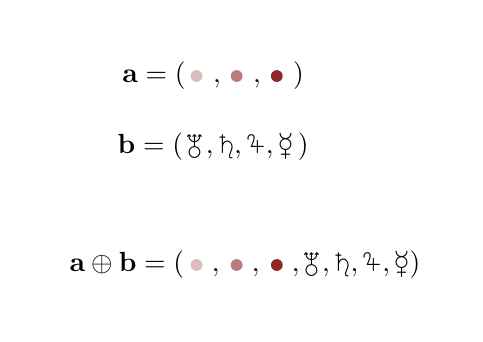
\begin{tikzpicture}[scale=0.3, thick]

\pgfmathsetmacro{\cx}{2}
\pgfmathsetmacro{\cy}{3}

\draw[white] (-8, -5) rectangle (10, 7);

\node[align=left] at (0, 5) { $\mathbf{a} = ( \quad, \quad, \quad  )$ };
\fill[light] (-0.9, 5) circle (0.25);
\fill[mid] (0.8, 5) circle (0.25);
\fill[dark] (2.5, 5) circle (0.25);

\node[align=left] at (0, 2) { $\mathbf{b} = ( \, \neptune, \saturn, \jupiter, \mercury \, )$ };

\node[] at (1.15, -3) 
{ $\mathbf{a} \oplus \mathbf{b} = ( \quad, \quad, \quad, \neptune, \saturn, \jupiter, \mercury)$ };
\fill[light] (-0.9, -3) circle (0.25);
\fill[mid] (0.8, -3) circle (0.25);
\fill[dark] (2.5, -3) circle (0.25);


\end{tikzpicture}

\end{document}  